\documentclass{school-22.101-notes}
\date{October 17, 2011}

\begin{document}
\maketitle

\subtopic{Summary of Quantum Numbers}
\begin{enumerate}
\item Orbital Angular Momentum Quantum Number $l$: integers, $0 \le l \le n$. A subset of j is the solution from orbital component. 
\item Total Angular Momentum Quantum Number $j$: integer steps, $|l-s|, \cdots, |l+s|$. It completely construct $l$ and $s$. 
\item $m_j$: $-j, \cdots j$ (includes 0 when j is an integer, and does not include 0 when j is a half-integer). It's degeneracy is $2j+1$. 
\end{enumerate}

\begin{table}[h!]
\begin{tabular}{|p{1.5in}|p{1.5in}|p{1.5in}|p{1.5in}|} \hline
 & $\Lhat$ & $\Shat$ &$\Jhat = \Lhat + \Shat$ \\ \hline
\multirow{3}{*}{Commutating Relations} &
   $\left[ \Lhat_x, \Lhat_y \right] = i \hbar \Lhat_z$ &  $\left[ \Shat_x, \Shat_y \right] = i \hbar \Shat_z$ &  $\left[ \Jhat_x, \Jhat_y \right] = i \hbar \Jhat_z$ \\
&  $\left[ \Lhat_y, \Lhat_z \right] = i \hbar \Lhat_x$ &  $\left[ \Shat_y, \Shat_z \right] = i \hbar \Shat_x$ &  $\left[ \Jhat_y, \Jhat_z \right] = i \hbar \Jhat_x$ \\
&  $\left[ \Lhat_z, \Lhat_x \right] = i \hbar \Lhat_y$ &  $\left[ \Shat_z, \Shat_x \right] = i \hbar \Shat_y$ &  $\left[ \Jhat_z, \Jhat_x \right] = i \hbar \Jhat_y$ \\ \hline
Quantum Numbers & $ l = 0,1,2,\cdots $ & $s = 0, 1/2, 1, \cdots$               & $ j =|l-s|,\cdots, |l+s|$ \\
(all in integer steps) & $-l \le m_l \le l  $  & $ -s \le m_s \le s$  & $-j \le m_j \le j$  \\ \hline
\multirow{2}{*}{Eigenvalues} 
& $\expect{L^2} = \hbar^2 l (l+1)$ 
& $\expect{S^2} = \hbar^2 s (s+1)$
& $\expect{J^2} = \hbar^2 j(j+1)$\\ 
& $\expect{L_z} = \hbar m_l$ 
& $\expect{S_z} = \hbar m_s$ 
& $\expect{J_z} =  \hbar m_j$  \\ \hline
\end{tabular}
\caption{Comparison of Quantum Numbers $l,s,j$}
\label{quantum-numbers}
\end{table}


\topic{Additions of Angular Momentum}
Examples:
\begin{enumerate}
\item $2e^-: \Lhat = \Lhat_1 + \Lhat_2 $ 
\item $ 1 e^-: \Jhat = \Lhat + \Shat$
\item \ce{^2H} = p+n: l =0. $\Jhat = \Shat_p + \Shat_n$. 
\end{enumerate}

\uline{Example 1: Adding Two Orbital Momentum:} we want to find the $(l,m)$ associated with $\Lhat= \Lhat_1 + \Lhat_2$ from the four quantum numbers $l_1, m_1, l_2, m_2$. 
\begin{itemize}
\item $\Lhat^2 = (\Lhat_1 + \Lhat_2)^2 $
\item $ \Lhat_z = \Lhat_{1z} + \Lhat_{2z} \Rightarrow m_{\mathrm{max}} = m_{\mathrm{1,max}} + m_{\mathrm{2,max}} = l_1 + l_2.$
$\fsp l_{\mathrm{max}} = m_{\mathrm{max}} = l_1 + l_2.$
\item $ \mbox{Total \# of independent states } N = (2 l_1 + 1) (2l_2 + 1) = \Sum_{l_{\mathrm{min}}}^{l_{\mathrm{max}}} (2l+1).$
$\fsp\Rightarrow l_{\mathrm{min}} = |l_2 - l_1 |.$ That is,
\eqn{ l = |l_2 - l_1|, \cdots , l_1 + l_2}
\end{itemize}

\uline{Example 2: Adding Two Electrons}

Given: $ 2e^-$, 1 $e^-$ \@ $l_1 = 1$, 1 $e^-$ \@ $l_2 = 2$. Answer: 
\begin{itemize}
\item $l = 1,2,3$.
\item $L = \hbar \sqrt{l (l+1)} = \hbar \sqrt{2}, \hbar \sqrt{6}, \hbar \sqrt{12}.$.
\item $N = \Sum_1^3 (2l+1) = 3 + 5 + 7 = 15$, or $N = 3 \times 5 = 15$. 
\end{itemize}

%%%%%%%%%%%%%%%%%% New Part: Nuclear Structure %%%%%%%%%%%%%%%%%%%%%%%%%%%%%%%%%
\lecture{Bound State of A Deuteron \label{2H-bound-state}}
We discuss a deuteron \ce{^2H} because it is the simplest bound state nucleus. We will show that a bound state problem can be reduced into the following steps:
\begin{itemize}
\item an eigenvalue problem (Section \ref{2H-eigenvalue});
\item an analytical relation and a quantitative relation between $V_0, \Gamma_0, E_0$ (Section \ref{2H-relation});
\item the spin dependence of the nuclear force (Section \ref{2H-spin}).
\end{itemize}
See more reference here\footnote{Liboff 10.5, Krane 4.1, 4.2, 4.4}.

\topic{Reduce Bound State Problem into Eigenvalue Problem \label{2H-eigenvalue}} 
\begin{enumerate}
\item Write out the Hamiltonian: 
\eqn{ \Hhat = \frac{1}{2 m_n} \phat_n^2 + \frac{1}{2 m_p} \phat_p^2 + V_{\mathrm{nuc}} (\uline{x}_n - \uline{x}_p ) }
in which 
\begin{align}
 V_{\mathrm{nuc}} (\uline{x}_n - \uline{x}_p ) &= \mbox{Potential interaction (only depends on the radial distance b/w the two particles)} \\
 (\uline{x}_p, \phat_p; \uline{x}_n, \phat_n) &= \mbox{State vectors of the two particles} 
\end{align}
We assume central potential. 6-degrees of freedom = \# of coordinates in the state vector

\item Convert to Center-of-Mass frame: 
\begin{align}
 H \to H_{\mathrm{CM}} + H_{\mathrm{Rel}}, \fsp \fsp (\uline{x}_p, \uline{p}_p; \uline{x}_n, \uline{p}_n) \to (\uline{r}, \uline{p}_{\mathrm{Rel}}; \uline{R}, \uline{p}_{\mathrm{CM}} ) \\
\begin{dcases*} 
\uline{R} = \frac{1}{m_n + m_p} (\uline{x}_p x_p + \uline{x}_n x_n) & C.M. position\\
\uline{r} = \uline{x}_p - \uline{x}_n & Relative position \\
\uline{p}_{\mathrm{CM}} = \uline{p}_{n} + \uline{p}_p & Momentum of CM \\
\uline{p}_{\mathrm{Rel}} = \frac{m_p \uline{p}_n - m_n \uline{p}_p}{m_n + m_p} & Momentum of coordinate relative to C.M \\
\end{dcases*}
\end{align}
Then a deuteon Hamiltonian becomes:
\begin{align}
\Hhat_d &= \overbrace{\frac{1}{2 \underbrace{M}_{=m_n + m_p}} \uline{\Phat}_{\mathrm{CM}}^2}^{ = \hat{E}_{\mathrm{CM}} \to  0} + \frac{1}{2 \underbrace{\mu}_{=\frac{m_n m_p}{m_n + m_p}}} \uline{\Phat}_{\mathrm{Rel}}^2 + V_{\mathrm{nuc}} (\uline{r}) \\
&= \frac{1}{2 \mu} \uline{\Phat}_{\mathrm{Rel}}^2 + V_{\mathrm{nuc}} (\uline{r}) = -\frac{\hbar^2}{2 \mu} \gradient_r^2 + V_{\mathrm{nuc}} (\uline{r}) 
\end{align}
in which $\gradient_r^2$ is Laplacian in relative coordinates. Now we've reduced the problem into a `single-particle' problem that described the reduced mass $\mu$ about the center of mass in $\uline{r}$. 

\item A qualitative evaluation of $V_{\mathrm{nuc}} (\uline{r})$ \footnote{Krane, p.80}: 
    \begin{enumerate}
    \item At short distances: very strong, overcome the Coulomb repulsion of protons in the nucleus; 
    \item At long distances: very week and negligible; 
    \item Some particles, like $e^-$, are immute to $V_{\mathrm{nuc}}$;
    \item The nucleus potential looks like Figure~\ref{nuclear-potential-radius}. 
    \begin{figure}
        \centering
        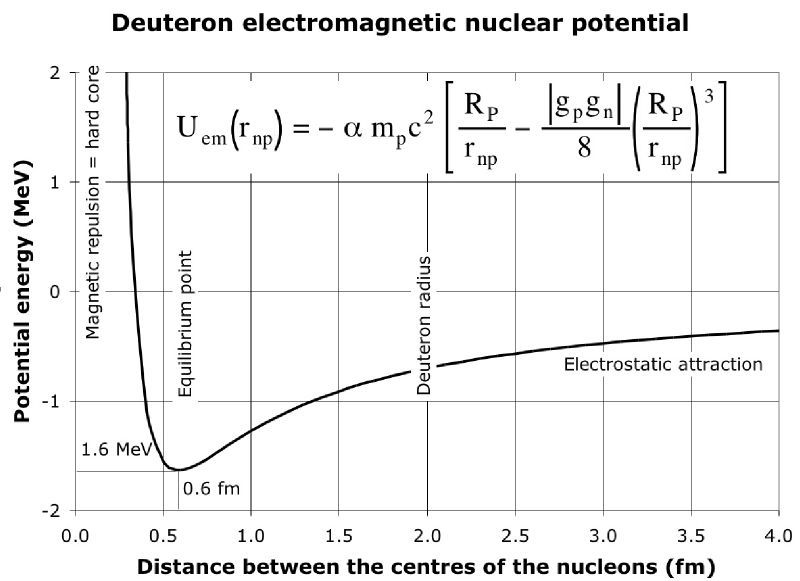
\includegraphics[width=3in]{images/deuteron/nuclear-potential-radius.png}
        \caption{Deuteron Electromagnetic Nuclear Potential\label{nuclear-potential-radius}}
    \end{figure}
    \end{enumerate}

\item A quantitative evaluation of $\uline{\gradient}_r^2$: 
\begin{align}
- \frac{\hbar^2}{2 \mu} \uline{\gradient}_r^2 &= - \frac{\hbar^2}{2 \mu} \left[ \pprn2 + \frac{2}{r} \ppr \right] + \frac{1}{2 r^2 \mu} \overbrace{ (-\hbar^2) \left[ \frac{1}{\sin \theta} \pptheta \left( \sin \theta \pptheta \right) + \frac{1}{\sin^2 \theta} \ppphin2 \right]}^{\to \Lhat^2}  \\
&= - \frac{\hbar^2}{2 \mu} \left[ \pprn2 + \frac{2}{r} \ppr \right] + \frac{\Lhat^2}{2 r^2 \mu} 
\end{align}

\item Now we have our eigenvalue problem:
\eqn{ \left[ - \frac{\hbar^2}{2 \mu} \left( \pprn2 + \frac{2}{r} \ppr \right) + \frac{\Lhat^2}{2 r^2 \mu} + V_{\mathrm{nuc}} (\uline{r})  \right] \psi_n (r, \theta, \phi) = E_n \psi_n (r, \theta,\phi) }

\item To evaluate the above eigenvalue problem, notice we have
\eqn{ \left[ \Lhat^2, \Hhat \right]   = \left[ \Lhat_z , \Hhat \right] = 0 }
suggesting that $\Lhat^2, \Lhat_z, \Hhat$ shares the same eigenstate, which is the spherical harmonics $Y_l^m (\theta, \phi)$. Then we can write the wave function as: 
\eqn{ \psi_n (r, \theta, \phi) = \psi_{n,l} (r) Y_l^m (\theta, \phi) }
Also we know 
\eqn{ \Lhat^2 Y_l^m = \hbar^2 l(l+1) Y_l^m }
Plug the eigenvalues of $\Lhat^2$ back into the eigenvalue problem: 
\eqn{ \left[ - \frac{\hbar^2}{2 \mu}\left( \pprn2 + \frac{2}{r} \ppr \right)  + \frac{\hbar^2 l(l+1)}{2 \mu r^2 } + V_{\mathrm{nuc}} (\uline{r}) - E_{n,l}  \right] \psi_{n,l} (r) Y_l^m (\theta, \phi) = 0 }
Notice that the above equation is only dependent on r, so we can cross out the $Y_l^m (\theta, \phi)$ term, and call the radial component of the state function $r \psi_n (r) = u_n (r)$: 
\eqn{  \boxed{ \left[ - \frac{\hbar^2}{2 \mu}  \pprn2  + \underbrace{\frac{\hbar^2 l(l+1)}{2 \mu r^2 } + V_{\mathrm{nuc}} (\uline{r}) }_{\to V_{\mathrm{eff}} (\uline{r})} - E_{n,l}  \right] u_n (r)  = 0 } }
In a sense, we defined a modified potential term $V_{\mathrm{eff}} (r)$ that takes into account the angular momentum effect.  
\begin{figure}
    \centering
    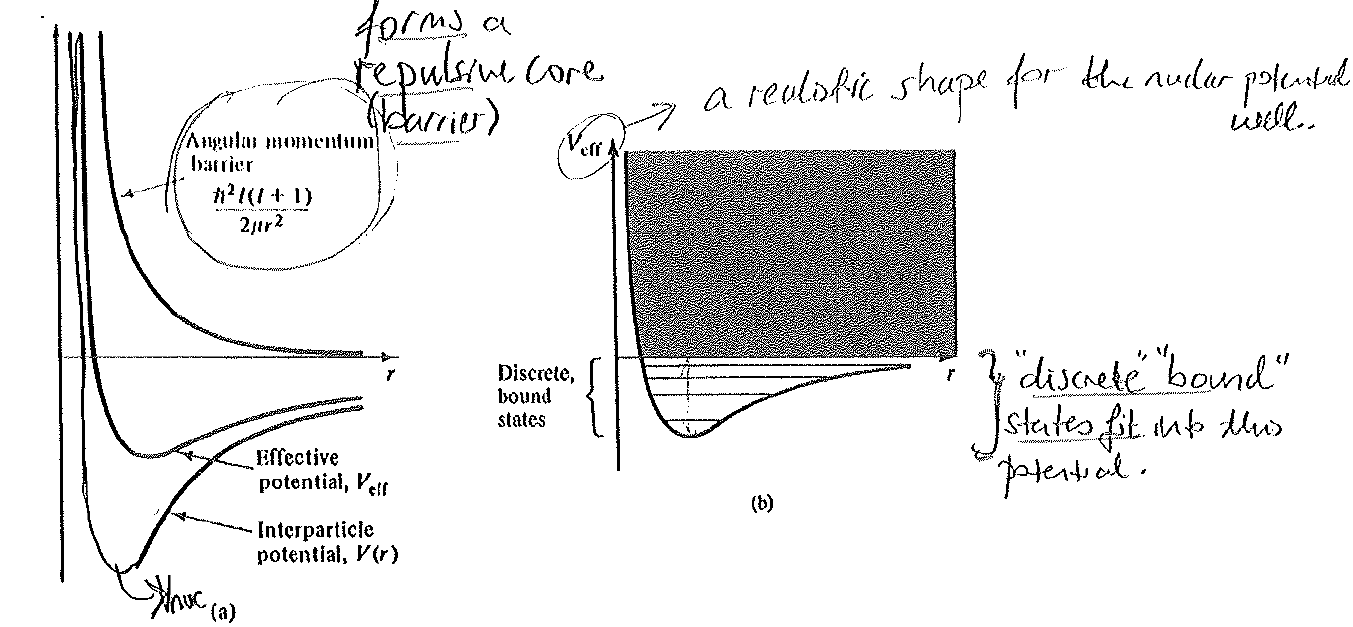
\includegraphics[width=4.5in]{images/deuteron/deutrium-V-eff.png}
    \\
    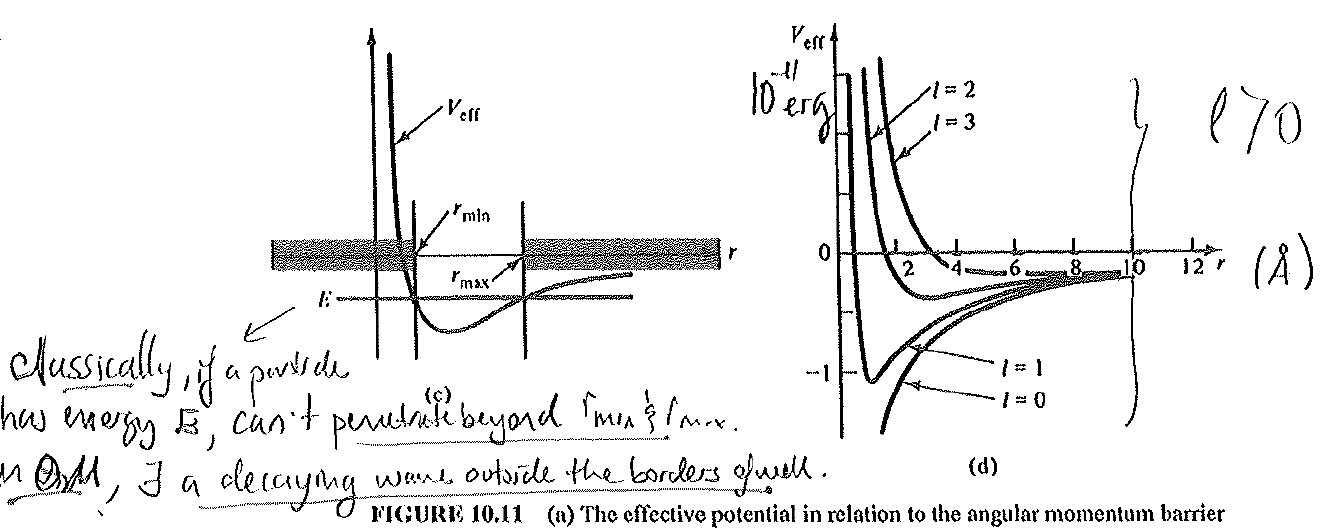
\includegraphics[width=4.5in]{images/deuteron/deutrium-V-eff-2.png}    
    \caption{$V_{\mathrm{eff}}$'s Effect on a Deutron}
    \label{V-eff}
\end{figure}
Interpretations of Figure~\ref{V-eff}:
\begin{enumerate}
\item Original $V_{\mathrm{nuc}} (r)$ is mostly attractive (negative); 
\item Angular momentum terms act as a repulsive barrier as it is positive;
\item $V_{\mathrm{eff}} (r)$ is still mostly attractive (negative), but weaker than $V_{\mathrm{nuc}} (r)$, In a word, \textcolor{blue}{$V_{\mathrm{eff}}$ lifts the potential up from the original $V_{\mathrm{nuc}}$, making the interaction weaker;} 
\item There are discrete bound states that fit into the potential. 
\end{enumerate}

\item Our goal: We've defined the particle potential. Now we are looking for the permitted energy levels $E_n$ that can fill in the potential. If we have a weaker potential, we can fit in less energy levels. Vice versa. From next class on we will solve this problem for deutrons. 
\end{enumerate}











\end{document}
